\documentclass[a4paper, 11pt]{article}
\usepackage[margin=1in, tmargin=1.5in, bmargin=1.5in]{geometry}
\usepackage{graphicx}
\graphicspath{ {./Images/} }
\usepackage{enumitem}
\usepackage{xcolor}
\usepackage{amsmath}
\usepackage{etoolbox}

\usepackage{makecell}
\usepackage{multirow}

\usepackage[edges]{forest}

\usepackage{pgfplots}
\pgfplotsset{compat=newest}
\usepackage{pgf-pie}
\usetikzlibrary{shapes.geometric, arrows}
%\tikzstyle{custom} = {>=stealth, font=\scriptsize}




\usepackage{varioref}
\usepackage{hyperref}
\hypersetup
{
	colorlinks=true, %set true if you want colored links
	linktoc=all,     %set to all if you want both sections and subsections linked
	linkcolor=blue,  %choose some color if you want links to stand out
	citecolor=teal,
	urlcolor=blue,
}
\usepackage{cleveref} % be sure to load 'cleveref' AFTER 'hyperref'
\crefname{subfigure}{}{}
\crefname{figure}{Fig.}{Figs.}

\usepackage{tablefootnote}
%\newcommand{\footref}[1]{\textsuperscript{\ref{#1}}}

\usepackage{lastpage,refcount}
\usepackage[english]{babel}
\usepackage{fancyhdr}
\pagestyle{fancy}
\renewcommand{\headrulewidth}{0pt}
\renewcommand{\footrulewidth}{0.4pt}
\fancyhf{}
%\fancyhead[C]{Assignment -- 3 on Metric Spaces}
%\fancyfoot[R]{\footnotesize Dept.\! of Mathematics\\Salesian College, Siliguri Campus}

\fancyfoot[L]{\ifnum\value{page}=\getpagerefnumber{LastPage}\small\color{gray!70!black}\emph{Compiled by:} Subhajit Paul and Debasmita Basu.
	\else \relax
	\fi}
\fancyfoot[R]{\ifnum\value{page}=\getpagerefnumber{LastPage}\small\color{gray!70!black}Page \thepage~of \getpagerefnumber{LastPage}
	\else \relax
	\fi}

\fancyfoot[C]{\ifnum\value{page}=\getpagerefnumber{LastPage} \relax
	\else \small\color{gray!70!black}Page \thepage~of \getpagerefnumber{LastPage}
	\fi}

\usepackage[labelformat=simple, labelsep=period]{caption}

\parskip1ex
\parindent0pt
\title{Cancer Alley and Data Visualization}
\author{Debasmita Basu}

\newcommand{\link}[2]{{\hyperref[#1]{\normalfont #2}}}
\allowdisplaybreaks[4]

\begin{document}
	\begin{titlepage}
		\maketitle
	\end{titlepage}
	\tableofcontents
	\thispagestyle{empty}
	\clearpage
	\setcounter{page}{1}
%
%
%Section 1: Objectives
%
%
\section{Objectives}
%\thispagestyle{fancy}
%
%Subsection 1.1: Mathematical/ Quantitative Goals
%
\subsection{Mathematical/Quantitative goals}
%
	By the end of the lesson, students will be able to:
	\begin{enumerate}[label=(\alph*), noitemsep]
		\item 
				Identify the different types of data.
		\item 
				Determine the best way to visualize data, based on their types.
		\item 
				Display numerical data in plots on a number line, including scatter plots, histograms, and box plots. (\hyperlink{http://www.corestandards.org/Math/Content/6/SP/B/4/}{CCSS.MATH.CONTENT.6.SP.B.4})
		\item 
				Summarize numerical data sets in relation to their context.\\ (\hyperlink{http://www.corestandards.org/Math/Content/6/SP/B/5/}{CCSS.MATH.CONTENT.6.SP.B.5})
		\item 
				Describing the nature of the attribute under investigation, including how it was measured and its units of measurement. (\hyperlink{http://www.corestandards.org/Math/Content/6/SP/B/5/b/}{CCSS.MATH.CONTENT.6.SP.B.5.B})
		\item 
				Giving quantitative measures of center (median and/or mean) and variability (interquartile range and/or mean absolute deviation), as well as describing any overall pattern and any striking deviations from the overall pattern with reference to the context in which the data were gathered. (\hyperlink{http://www.corestandards.org/Math/Content/6/SP/B/5/c/}{CCSS.MATH.CONTENT.6.SP.B.5.C})
	\end{enumerate}
%
%Subsection 1.2: Environmental justice goal
%
\subsection{Environmental justice goals}
%
	By the end of the lesson, students will be able to:
	\begin{enumerate}[label=(\alph*), noitemsep]
		\item 
				Interpret data and identify the disproportionate impact of environmental issues on African-American people.
		\item 
				Identify how cancer alley, creates a form of environmental racism, and poses serious and disproportionate health threats on people of color.
	\end{enumerate}
%
%
%Section 2: Understanding the Issue
%
%
\section{Understanding the Issue}
%
%
	In the southern state of Louisiana, along the lower Mississippi River, nearly 150 oil refineries, plastics plants, and chemical facilities are located between New Orleans and Baton Rouge. Environmentalists call this 85-mile-long stretch the Chemical Corridor or Cancer Alley, while industrialists adopted the name Industrial corridor to describe this region. As the name suggests, residents of this area are 50 times more susceptible to get cancer compared the national average \cite{SM11}, in some parishes the chance being even higher. In a 1991 interview, Amos Favorite, a resident of Ascension Parish on the Cancer Alley stated,
	\begin{quotation}
		I lost my Uncle James Barber and his son Israel $\dots$ I lost another uncle, Jorden Favorite, his wife, Pipine, and their son Isaac. Then there was another uncle, Herbert Favorite. My cousins Lizzie and Emily died in their 40s. Then there was my aunt’s husband, Josene LeBlanc $\dots$ Our people used to live to be 95, 100, years old $\dots$ Now even the young people are dyin’. [Reed 1991]
	\end{quotation}
	This is the reality of one of many families living on the Cancer Alley.
%
	\begin{figure}[h!]
		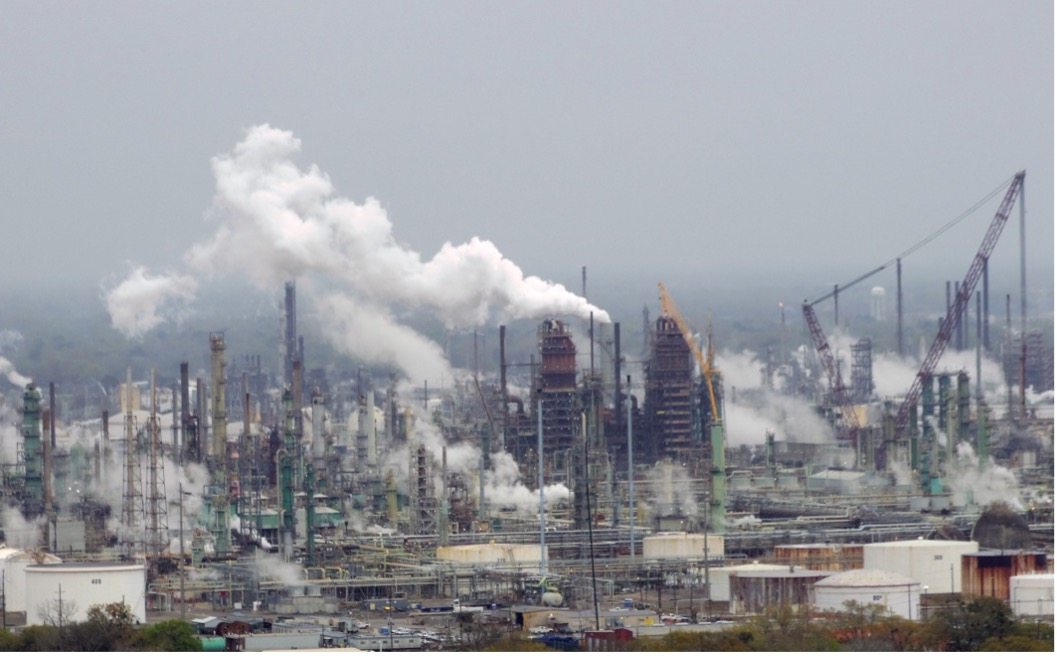
\includegraphics[width=\linewidth]{Picture 1.jpg}
		\caption{Chemical facilities in Baton Rouge, Source: \href{https://en.wikipedia.org/wiki/Baton_Rouge_Refinery}{Wikipedia} is licensed with \href{https://creativecommons.org/publicdomain/zero/1.0/}{CC0 1.0}}
	\end{figure}
%	
	Louisiana is one of the highest producers of hazardous waste materials in the United States (Allen, 2006). Every year, the chemical factories located in the state, especially on the cancer alley releases vast amount of carbon-dioxide and millions of pounds of poisonous chemicals, thus jeopardizing the health of the residents and the people working in the chemical facilities (Singer, 2011). The toxic chemicals do not only pollute the air, but unsustainable waste disposal systems, chemical release from factories, and seepage of fertilizers and pesticides from agricultural production also contaminate drinking water. A study by Gottlieb, Carr, and Morris (1981) reported that the residents of cancer alley, who get their drinking water from Mississippi river are 2.1 times more susceptible to rectal cancer compared to those who depends on an alternate source for their drinking water. Apart from cancer, skin inflammation, significant respiratory problems, and a range of other health threats have also been predominant among the people living in the cancer alley (Lerner, 2006).\\[1ex]
%	
	Although the cancer is highly predominant among all the people residing in the Cancer Alley, African American people bear a disproportionate burden of cancer mortality compared to the other racial counterparts. Between 1995 and 2006, while the cancer mortality rate of the white men and women were 250 and 167 per 100,000 population, the mortality rate of African American men and women were 395 and 214 per 100,000 population respectively (Singer, 2011). One of the reasons behind this glaring difference in the cancer mortality rate is probably because most of the chemical factories and hazardous waste sites on the Cancer Alley are established in areas which are heavily resided by impoverished, people of color. According to Castellón (2021) “there is little evidence that communities of color move to sites where toxic waste facilities and landfills are located. Rather, toxic waste sites are often sited in primarily poor and African American neighborhoods” (p. 16). While affluent white communities are often able to "leverage their economic and political clout" to prevent establishment of unwanted facilities in their neighborhoods (Bullard, 2019), lack of political support and money, disable people of color to relocate or afford legal representations to fight big industrial facilities moving to their localities (Castellón, 2021). Such disproportionate burden of environmental harms on a particular socio-economic and racial group is called environmental racism (Bullard, 2018).\\[1ex]
%	
	In this lesson, we will explore the topic of environmental racism through the case of cancer alley. We will extract racial composition data of people living along the 85-mile-long stretch of the Chemical Corridor and use data visualization to compare and identify the disproportionate impact of the chemical factories on African American people.
%
%Subsection 2.1: Supplementary materials on Cancer Alley
\subsection{Supplementary materials on Cancer Alley}
%
	\begin{itemize}[noitemsep]
		\item \href{https://www.youtube.com/watch?v=ZB8CbDG7gpk}{Why This Town Is Dying From Cancer | AJ+}
		\item \href{https://www.youtube.com/watch?v=MGNtMkFJkKg}{Cancer risk in Louisiana town nearly 50 times higher than national average}
		\item \href{https://www.youtube.com/watch?v=XAFD-0aMkwE}{One reason why coronavirus hits Black people the hardest}
		\item \href{https://www.youtube.com/watch?v=9hE3SyXr9bw}{EPA 20th Anniversary Environmental Justice Video Series: Dr. Beverly Wright}
	\end{itemize}
%
%
%Section 3: Understanding the Math
%
%
\section{Understanding the Mathematics}
%
%Subsection 3.1: What is data visualization
%
\subsection{What is data visualization}
%
	Data visualization is a way to graphically represent data and information by using visual elements such as charts, graphs, and maps. The purposes of data visualizations are to summarize, compare, reveal patterns, and notice anomalies present in the data; in other words, data visualization makes data more understandable to an individual.
%
%Subsection 3.2: Why is data visualization important?
%
\subsection{Why is data visualization important?}
%
	In the world of big data, where we have access to a large amount of information, it is an essential skill for an individual to learn to handle a significant volume of data and devise a quick and effective way to present the data in meaningful ways to others. Data visualization is a tool that serves such purposes. It provides an intuitive way to visualize and understand trends, outliers, clusters, and patterns in given data sets. Data visualization also helps us compare different data sets and prompts us to raise questions that stimulate research and suggest ideas. It offers a meaningful way to tell a story from data but with a purpose.
%
%Subsection 3.3: Data classification and visualizations
%
\subsection{Data classification and visualizations}
%
	Once you collect or obtain a data set, you need to choose which form of data visualization(s) would be appropriate for your data. But before you can determine the best form of data visualization, you need to classify your data. The nature of your data would help you determine the possible forms of visualizations. In the following section, we will discuss the different types of data with examples.
%
\subsubsection{Data types}
%
	Let’s say you are conducting a neighborhood welfare survey. The survey aims to learn about the different issues the residents are concerned about and want the local authorities to address immediately. The survey contains a combination of ten closed and open-ended questions. For details about the survey, see \vref{pictureX}. Overall, the survey questions collected two types of data: non-numeric (Questions 1, 2, 5, 6, 9) and numeric (Questions 3, 4, 7, 8, 10), based on which the data can be broadly classified into two types: categorical data and quantitative data.
	\begin{figure}[h!]
		\centering
		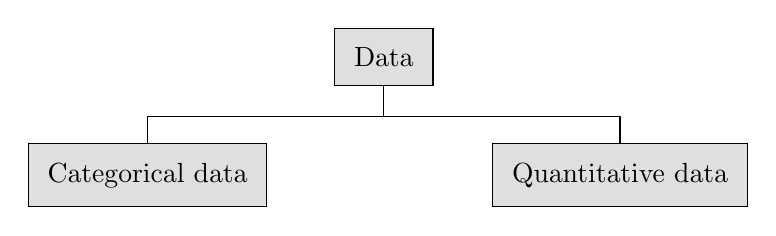
\begin{tikzpicture}[declare function={a=-0.75;}]
			\draw (0,0) -- (0,a) (-3,a) -- (3,a) -- (3,2*a) (-3,a) -- (-3,2*a);
			\node [fill=gray!25, rectangle, inner sep=7pt, draw=black] at (0,0) {Data};
			\node [fill=gray!25, rectangle, inner sep=7pt, draw=black] at (-3,2*a) {Categorical data};
			\node [fill=gray!25, rectangle, inner sep=7pt, draw=black] at (3,2*a) {Quantitative data};
		\end{tikzpicture}
		\caption{}
	\end{figure}
%
	\paragraph{Categorical data:}
	Data that are non-numeric or qualitative in nature, and that can be classified into different categories; are called Categorical Data. For example, question 2 of the survey asked the respondents, “What are some issues, if at all, in your neighborhood that concerns you the most?” It provided the respondents with nine non-numeric options to choose from, 
		\begin{enumerate}[label=(\alph*), noitemsep]
		\item 
		Lack of proper waste disposal system
		\item
		Air Pollution
		\item
		Access to healthy drinking water
		\item
		Lack of green spaces/ parks/ playground
		\item
		Availability of healthcare system
		\item
		Risk of flooding/ forest fire
		\item
		Access to grocery stores/ neighborhood market
		\item
		Unsafe road conditions
		\item
		Others
		\end{enumerate}
		
Each response forms a category; hence, question 2 collected categorical data. 
%
	\paragraph{Quantitative Data:}
	Data that are numeric in nature and hence quantifiable, are called quantitative data. Question 7 in the survey asked the respondents, “How many people live in your household?” Such variables “Number of people” would record data that are numbers; hence are called quantitative data. 
%
	\begin{figure}[h!]
		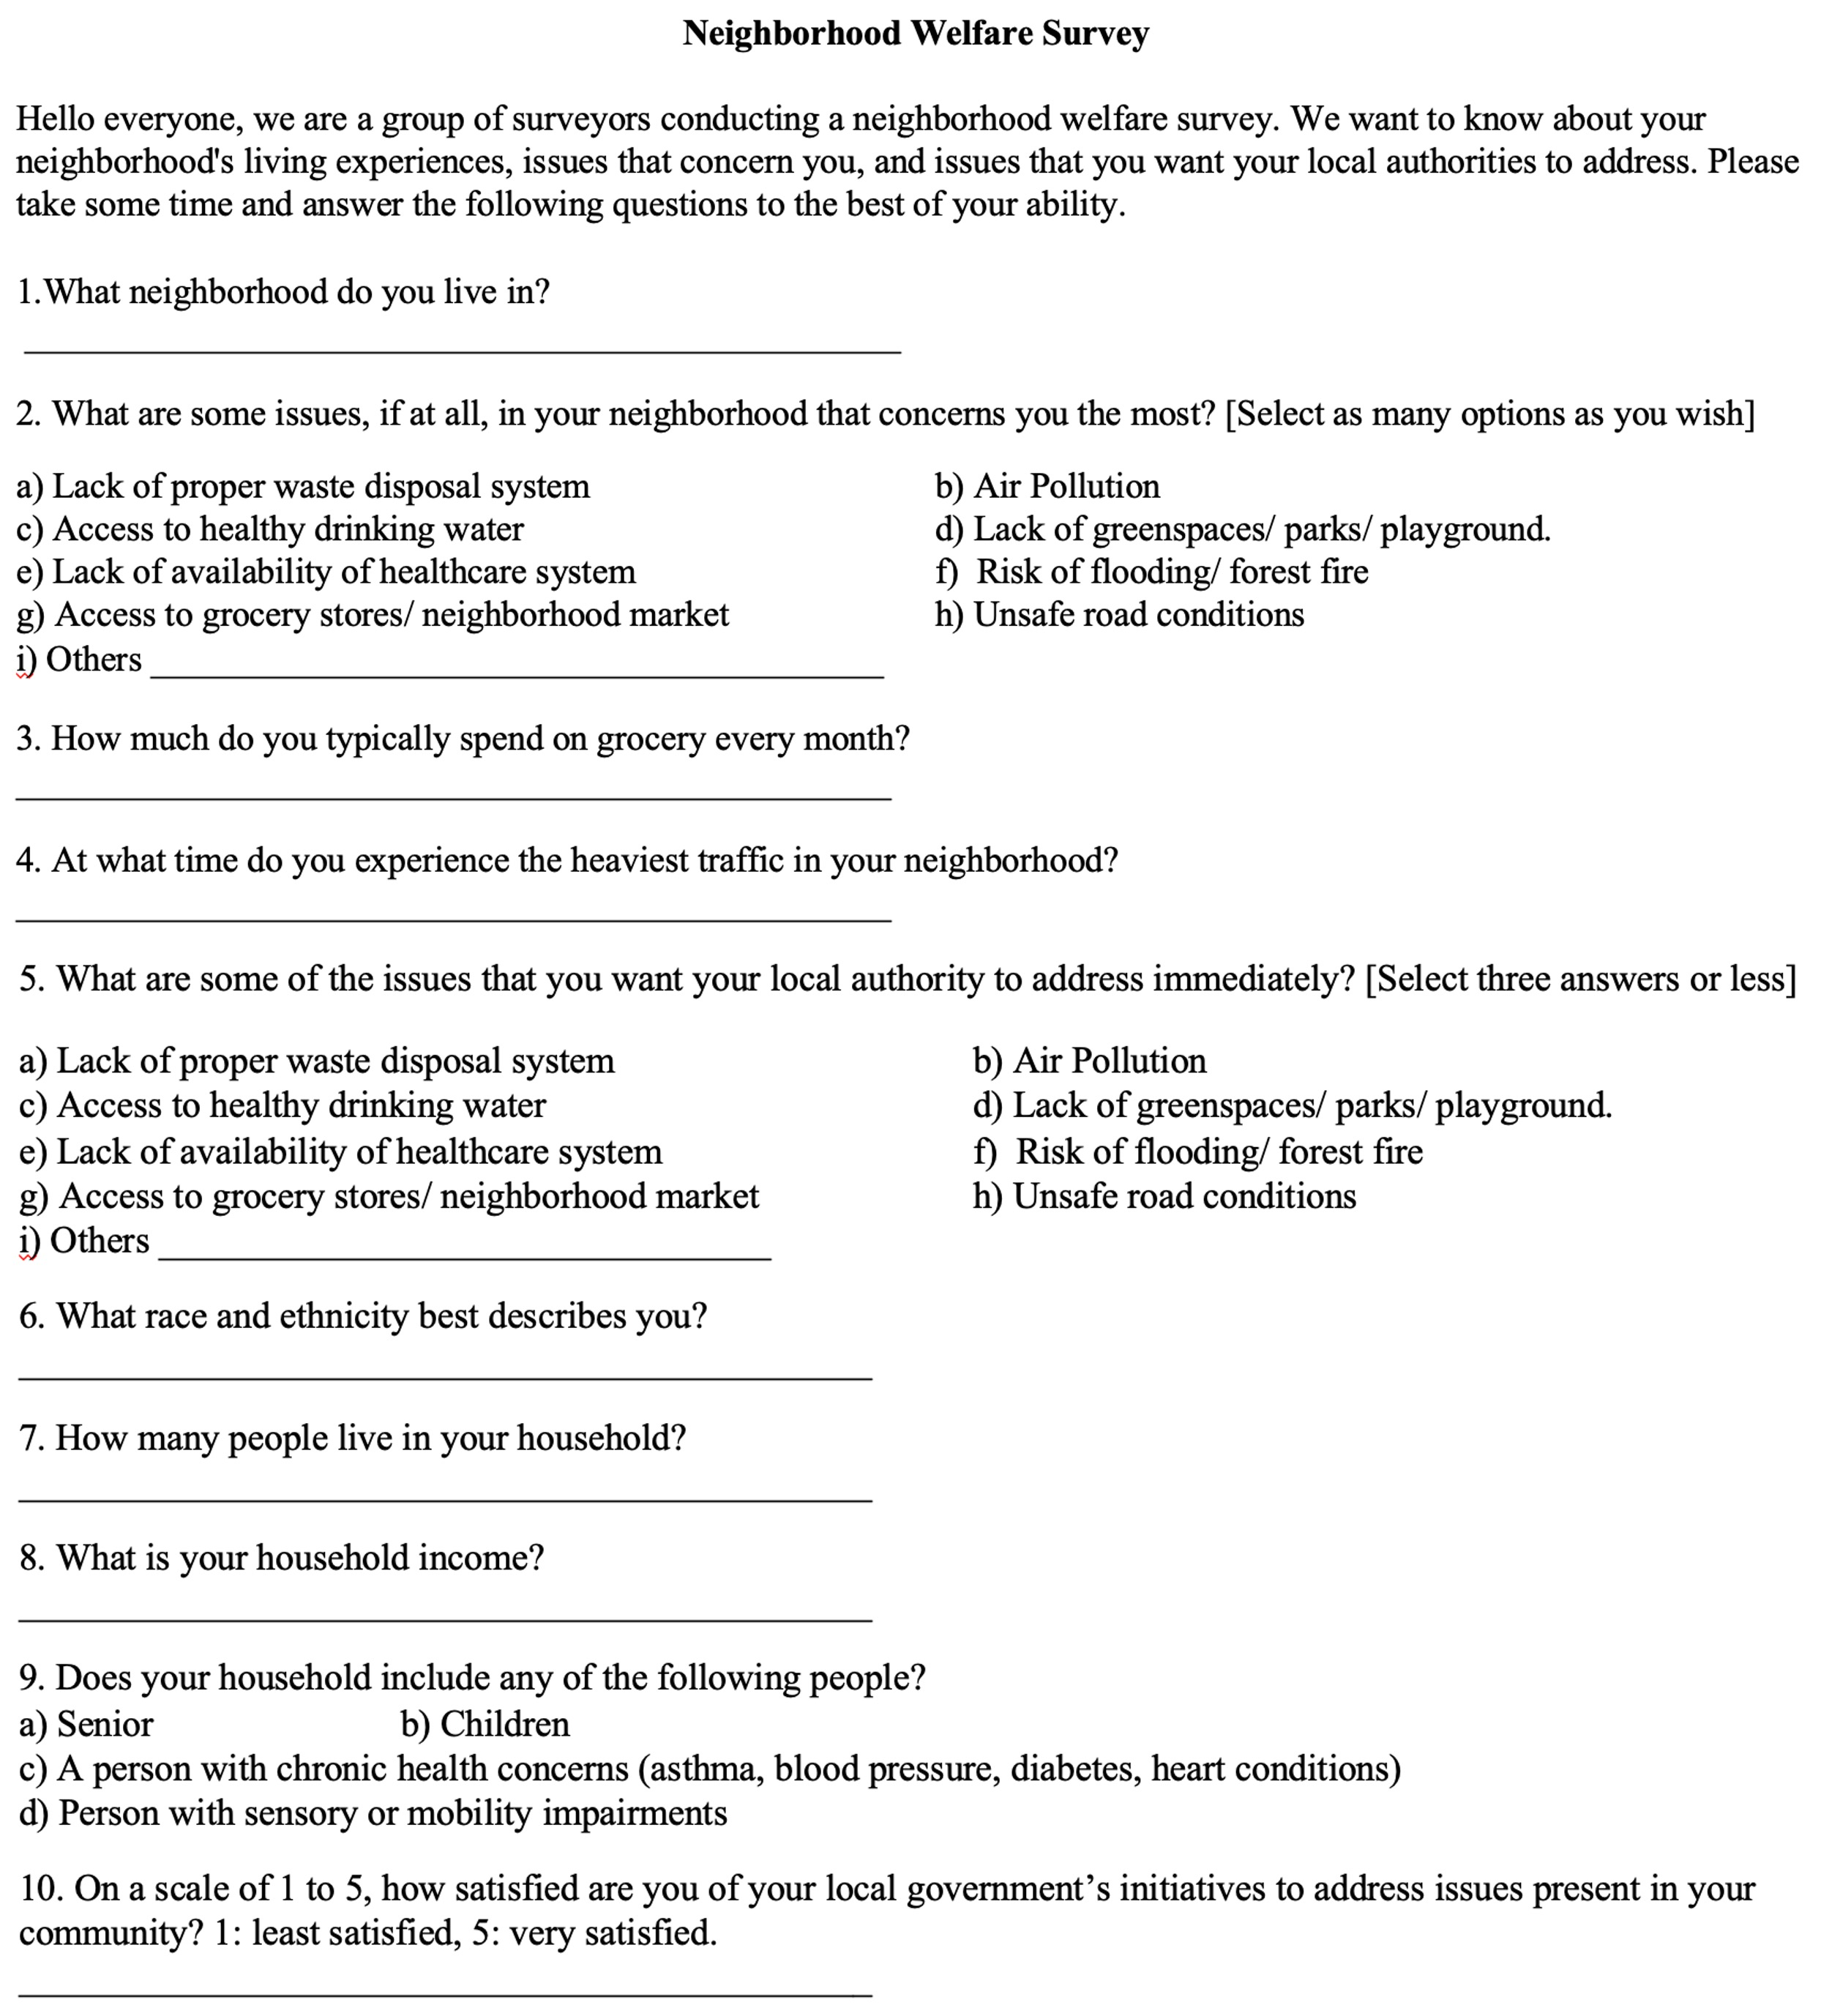
\includegraphics[width=\linewidth]{Neighborhood welfare survey.jpg}
		\caption{Neighborhood welfare survey}
		\label{pictureX}
	\end{figure}
%
	\paragraph{}Categorical data can further be classified into two types: nominal data and ordinal data.
%	
	\paragraph{Nominal data:} Let us refocus on Question 2 of the survey, “What are some issues, if at all, in your neighborhood that concerns you the most?” The question provided the respondents with nine non-numeric options,
	\begin{enumerate}[label=(\alph*), noitemsep]
		\item 
		Lack of proper waste disposal system
		\item
		Air Pollution
		\item
		Access to healthy drinking water
		\item
		Lack of green spaces/ parks/ playground
		\item
		Availability of healthcare system
		\item
		Risk of flooding/ forest fire
		\item
		Access to grocery stores/ neighborhood market
		\item
		Unsafe road conditions
		\item
		Others
		\end{enumerate}
	These nine options form nine categories whose order is not essential. Such qualitative data, which can be classified into different categories, but the order of the categories is not important, are called Nominal Data.\\[1ex]
Nominal data can be counted and hence it can be used to calculate the number of times or the percentage of times a particular category has been selected. No other meaningful mathematical operations can be performed on Nominal Data. 
%	
	\paragraph{Ordinal Data:} Categorical data, where the order of the categories is important, is called Ordinal data. Question 10 of the survey asked the respondents, “How satisfied are you with your local government’s initiatives to address issues present in your community?” It provided the respondents with five non-numeric options: Extremely satisfied, satisfied, Average, Dissatisfied, and Extremely Dissatisfied. Here, the five options create five categories, and there exists a natural ordering between these categories. Hence such data is Ordinal in nature.\\[1ex]
	Like nominal data, you can count ordinal data and use them to calculate the number of times or the percentage of times a particular category has been selected. However, some disagreement exists about whether you can perform any other mathematical operations, especially calculate the average, with Ordinal Data. When Ordinal data is in non-numeric form, you cannot calculate its average and measure the average response of the respondents. However, sometimes numbers are assigned to the different categories of Ordinal data for easier data entry and analysis (5: Extremely satisfied, 4: satisfied, 3: Average, 2: Dissatisfied, and 1: Extremely Dissatisfied). Although these numbers do not have any true mathematical value, you can often use these numbers to calculate the average response under the assumption that the difference in degree between consecutive categories is approximately equal.
%
	\paragraph{}Quantitative data can also be classified into two types: interval and ratio data.
%	
	\paragraph{Interval data:} Let us start with an example. Question 4 of the survey asked the respondents, “At what time do you experience the heaviest traffic in your neighborhood? Imagine how a respondent would respond to that question? 7:30 AM? 8 AM? All the responses will record the time of the day. Such data is numerical and will be classified as Interval Data.\\[1ex]
	Interval data are numerical, and as a result, the interval between the consecutive points of measurement are uniform. Whether someone experiences the heaviest traffic at 8 AM or 8:30 AM, or 9 AM, the difference between all the three timings is consistently 30 minutes or .5 hours.\\[1ex]
	Since interval data is numeric, you can perform any mathematical operation, but interval data does not have any meaningful zero. For example, suppose Sunday at midnight, there was an accident in your neighborhood, and as a result, there was massive traffic in your neighborhood. One way to measure the timing is through a 24-hour clock and say that your neighborhood experienced unusual traffic at 0:00 AM on Sunday. Here zero does not mean that there is an absence of time. Zero is just the measure of the time of the day using a 24-hour clock.
%
	\paragraph{Ratio data:} To understand Ratio Data, let us get back to question 7, where the survey asked the respondents, “How many people live in your household?” Unlike Interval data, in this question, if you say that zero people live in the household, it means that no people live in the household. So, in Ratio data, the value zero indicates an absence of a measure.\\[1ex]
	Like interval data, ratio data is numeric in nature. Hence, the interval between the consecutive points of measurement is uniform, and you can perform any mathematical operations on it.
%
	\begin{figure}
		\centering
		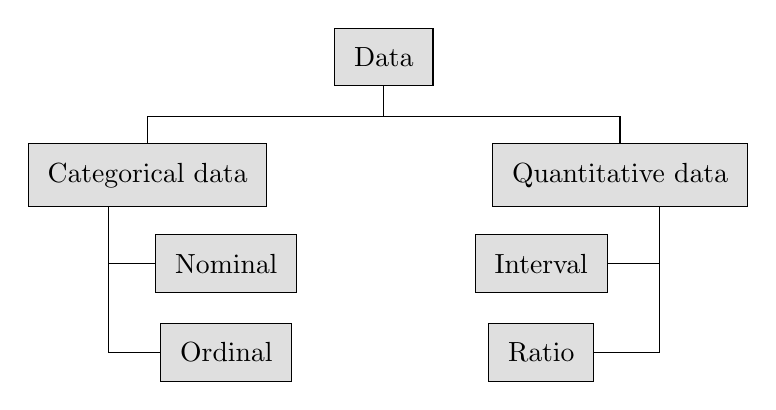
\begin{tikzpicture}[declare function={a=-0.75;}]
			\draw (0,0) -- (0,a) (-3,a) -- (3,a) -- (3,2*a) (-3,a) -- (-3,2*a) (-3.5,2*a) -- (-3.5,5*a) -- (-2.5,5*a) (-2.5,3.5*a) -- (-3.5,3.5*a) (3.5,2*a) -- (3.5,5*a) -- (2.5,5*a) (2.5,3.5*a) -- (3.5,3.5*a);
			\node [fill=gray!25, rectangle, inner sep=7pt, draw=black] at (0,0) {Data};
			\node [fill=gray!25, rectangle, inner sep=7pt, draw=black] at (-3,2*a) {Categorical data};
			\node [fill=gray!25, rectangle, inner sep=7pt, draw=black] at (3,2*a) {Quantitative data};
			\node [fill=gray!25, rectangle, inner sep=7pt, draw=black] at (-2,3.5*a) {Nominal};
			\node [fill=gray!25, rectangle, inner sep=7pt, draw=black] at (-2,5*a) {Ordinal};
			\node [fill=gray!25, rectangle, inner sep=7pt, draw=black] at (2,3.5*a) {Interval};
			\node [fill=gray!25, rectangle, inner sep=7pt, draw=black] at (2,5*a) {Ratio};
		\end{tikzpicture}
		\caption{}
	\end{figure}
	%
\subsubsection{Exercises}
%
Go to the survey: Neighborhood welfare survey, and identify the survey questions that gather data of the following types:
\begin{enumerate}[label=(\alph*), noitemsep]
		\item 
				Quantitative
		\item 
				Nominal
		\item 
				Ratio
		\item 
				Interval
		\item 
				Categorical
		\item 
				Ordinal
	\end{enumerate}
%
\subsubsection{Choosing data visualizations}
%
	Once you identify your data type, you can choose your data visualizations accordingly. For guidance, see \vref{table1}
	\begin{table}[h!]
		\def\arraystretch{1.25}
		\centering
		\begin{tabular}{|*{4}{c|}}
			\hline\hline
			\makecell[c]{\textbf{Number of}\\\textbf{variables}}	&	\multicolumn{2}{c|}{\textbf{Data types}}	&	\textbf{Visualisations}\\
			\hline\hline
			\multirow{2}{0.5in}{1}	&	\multirow{2}{1.5in}{Categorical data}	&	Nominal data	&	\makecell[c]{Pie chart\\Bar graph}\\
			\cline{3-4}
			&	&	Ordinal data	&	\makecell[c]{Pie chart\\Bar graph}\\
			\hline
			\multirow{2}{0.5in}{1}	&	\multirow{2}{1.5in}{Quantitative data}	&	Interval data	&	\makecell[c]{Histogram\\Bar graph}\\
			\cline{3-4}
			&	&	Ratio data	&	\makecell[c]{Histogram\\Bar graph}\\
			\hline
			\multirow{2}{0.5in}{2}	&	\multirow{2}{1.5in}{Quantitative data}	&	Interval data	&	Scattered plot\\
			\cline{3-4}
			&	&	Ratio data	&	Scattered plot\\
			\hline
		\end{tabular}
		\caption{Data Types and Visualizations}
		\label{table1}
	\end{table}
%
	A brief account of each of the data visualization is given below:
%
	\paragraph{Pie chart:} A pie chart is a visual tool that graphs categorical data and helps one understand the part-to-a-whole relationship. Visually a pie chart is circular in shape that is divided into sectors, where each sector represents the number or percentage of times an observation or category has been selected. The pie chart given in Figure~\ref{fig:Pie}, represents the the number or percentage of times respondents expressed concerns about their neighborhood issues. Each sector of the pie chart represents a distinct category, that is a particular neighborhood issue. \\[1ex]
	The pie chart given in Figure~\ref{fig:Pie} shows that 
	\begin{enumerate}[label=(\alph*), noitemsep]
		\item 
	15\% times respondents expressed their concerns about improper waste disposal system, 
		\item 
	10\% times respondents expressed their concerns about air pollution, 
	\item 
	20\% times respondents expressed their concerns about access to healthy drinking water, 
	\item 
	6\% times respondents expressed their concerns about lack of greenspaces/ parks/ playgrounds, 
	\item 
	14\% times respondents expressed their concerns about availability of healthcare system, 
	\item 
	2\% times respondents expressed their concerns about risk of flooding/ forest fire, 
	\item 
	11\% times respondents expressed their concerns about access to grocery stores/ neighborhood market, 
	\item
	18\% times they expressed their concerns about unsafe road conditions, and
	\item
	4\% times they expressed their concerns about other neighborhood issues not included in the list.
	\end{enumerate}
	The important thing to know about a pie chart is that the bigger the area of the sectors, the greater the values they represent. That means, in the given pie chart, since the area of the sector representing “Access to healthy drinking water” is the highest (20\% of the total area), you can conclude that out of the nine given issues, the respondents chose "Access to healthy drinking water” the maximum number of times. To be precise, 20\% of the times respondents said that they were concerned about healthy drinking water. Likewise, the area of the sector representing “Risk of flooding/ forest fire” is the smallest (2\% of the total area), the pie chart suggests that only 2\% of times respondents said that they were concerned about flooding and forest fire. 
	\begin{figure}[h!]
	\centering
%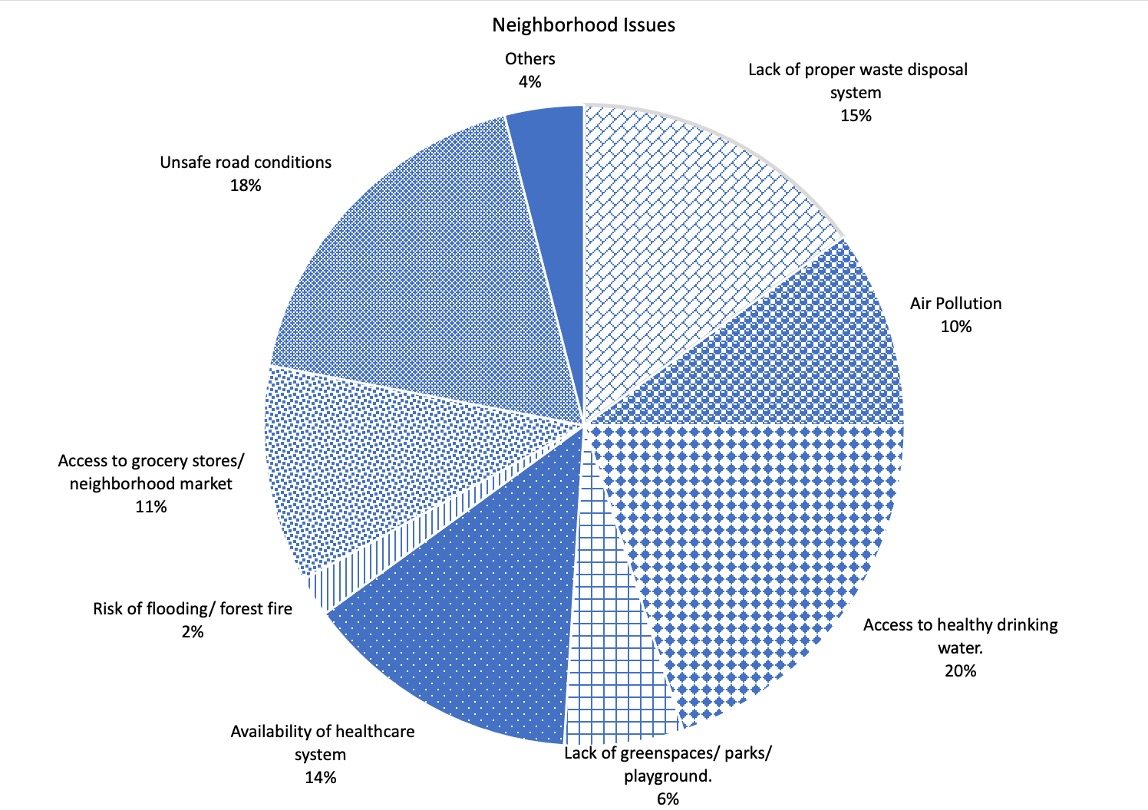
\includegraphics[width=105mm]{Pie_new.jpg}
	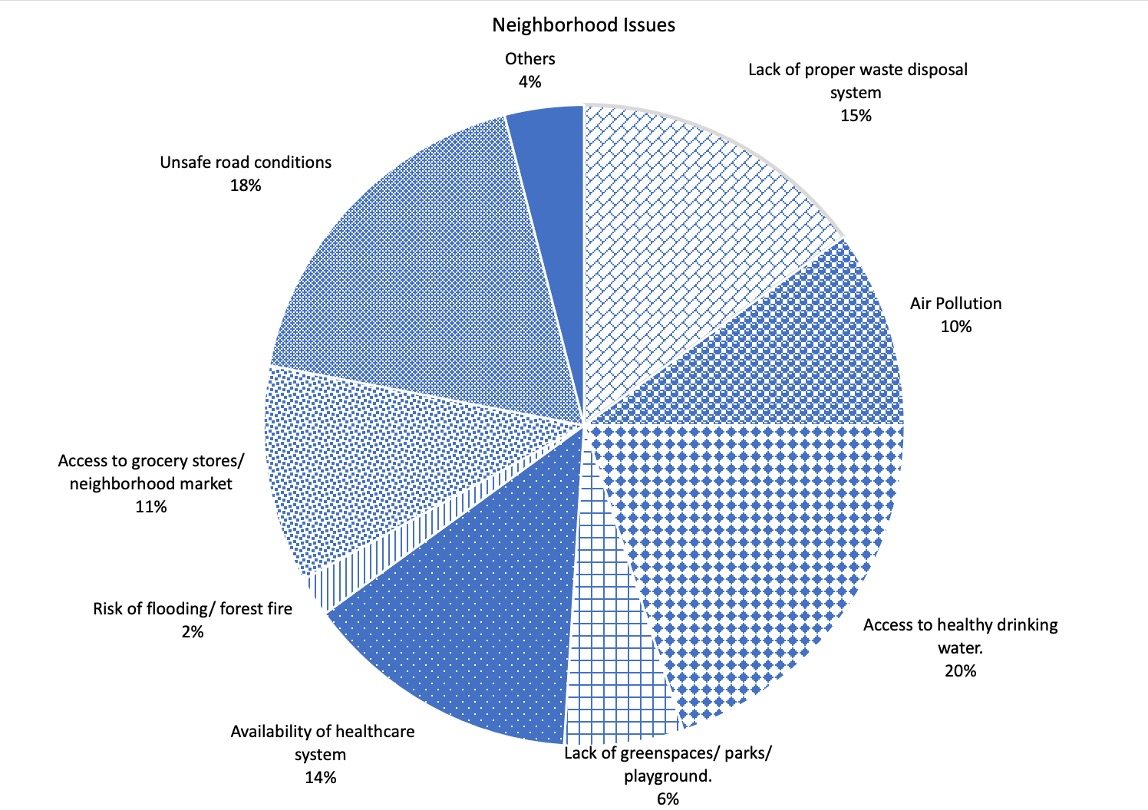
\includegraphics[width=\linewidth]{Pie_new.jpg}
		\caption{Pie Chart representing the different neighborhood related issues that the survey respondents are concerned about} 
		\label{fig:Pie}
	\end{figure}
%
    \paragraph{How to create a pie chart?}
    A pie chart is usually drawn to graph categorical data. To create a pie chart,
    \begin{enumerate}[label=(\alph*), noitemsep]
			\item
    First, create a frequency distribution table, where you will note how many times a particular category has been repeated. For example, question 2 of the "Neighborhood welfare survey" asked the respondents to indicate all the neighbourhood-related issues they were concerned about. The question provided the respondents with nine options. Each option would be considered as a category. Based on the responses, if you find that 200 responses have been collected, and 30 of them indicate lack of a proper waste disposal system, then the corresponding frequency would be 30. Likewise, if 20 out of 200 responses indicate respondents' concern about air pollution, then the corresponding frequency would be 20. 
    \begin{figure}[h!]
	\centering
	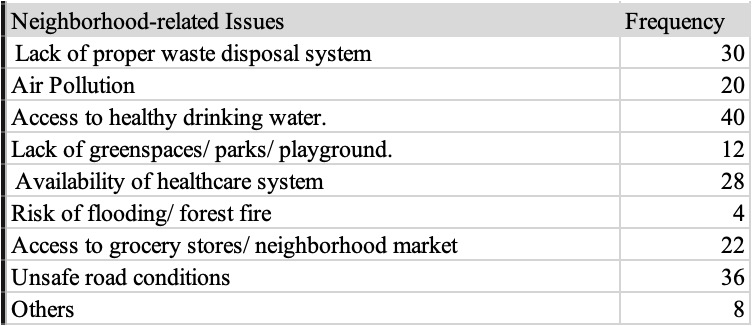
\includegraphics[width=\linewidth]{Freq_dist.jpg}
		\caption{Frequency distribution table of neighborhood-related issues} 
	\end{figure}
   \item
   Next, calculate the relative frequency of each category and their corresponding percentage. To calculate the relative frequency of each category, divide the frequency of each category by the total number of responses. For example, the relative frequency of lack of a proper waste disposal system = $\frac{30}{200}$ = $\frac{3}{20}$
   Likewise, the relative frequency of air pollution = $\frac{20}{200}$= $\frac{1}{10}$
   To calculate the corresponding percentages, multiply the relative frequencies by 100. For example, the percentage corresponding to lack of a proper waste disposal system = $\frac{3}{20}\times100$ = 15\%\\[1ex] 
   That means, 15\% of the times respondents expressed their concerns about lack of a proper waste disposal system in their neighborhood. 
   \begin{figure}[h!]
	\centering
	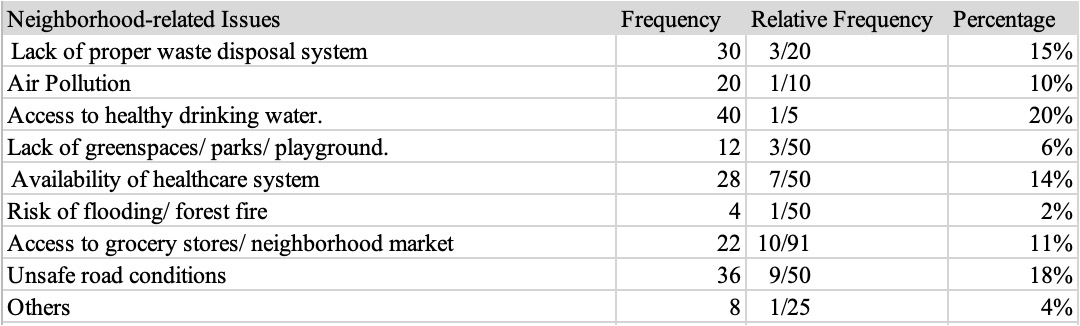
\includegraphics[width=\linewidth]{Percent.jpg}
		\caption{Relative frequency distribution table of neighborhood-related issues and their corresponding percentages} 
	\end{figure}
	\item
	Finally, once the percentages are calculated, create the pie chart. Divide the circle into sectors, where each sector represents a category. The relative area of each sector must match the percentage of time a particular category has been selected. For example, since 15\% of the times respondents expressed their concerns about the lack of a proper waste disposal system, the area of the sector representing "lack of a proper waste disposal system" is 15\% of the total area of the pie chart. Refer to Figure~\ref{fig:Pie} 
    \end{enumerate}
    
	\paragraph{Bar graph:} A bar graph is a visual tool that uses bars to compare data belonging to different categories. In the bar graph given given in Figure~\ref{fig:Bar}, each bar represents the number of times respondents raised concerns about different issues in their neighborhoods. As the visualization suggests, 15 respondents expressed their concerns about lack of proper waste disposal system, 10 respondents expressed their concerns about air pollution, 20 respondents expressed their concerns about access to healthy drinking water, six respondents expressed their concerns about lack of greenspaces/ pars/ playgrounds in the neighborhood, 14 respondents expressed their concerns about availability of healthcare system, 2 respondents expressed their concerns about forest fire and flooding, 11 respondents expressed their concerns about access to grocery stores and neighborhood markets, 18 respondents expressed their concerns about unsafe road conditions, and four respondents expressed their concerns about other issues in the neighborhood that are not included in the list.\\[1ex] 
	The important thing to know about a bar graph is that the longer/ taller the bars are, the greater the values they represent. That means, in the given bar chart, since the height of the bar representing “Access to healthy drinking water” is the highest, you can conclude that most of the respondents, twenty to be precise, said that they were concerned about healthy drinking water. Likewise, the height of the “Risk of flooding/ forest fire” bar suggests that minimum number of respondents, two to be precise, said that they were concerned about flooding or forest fire.
	\begin{figure}[h!]
		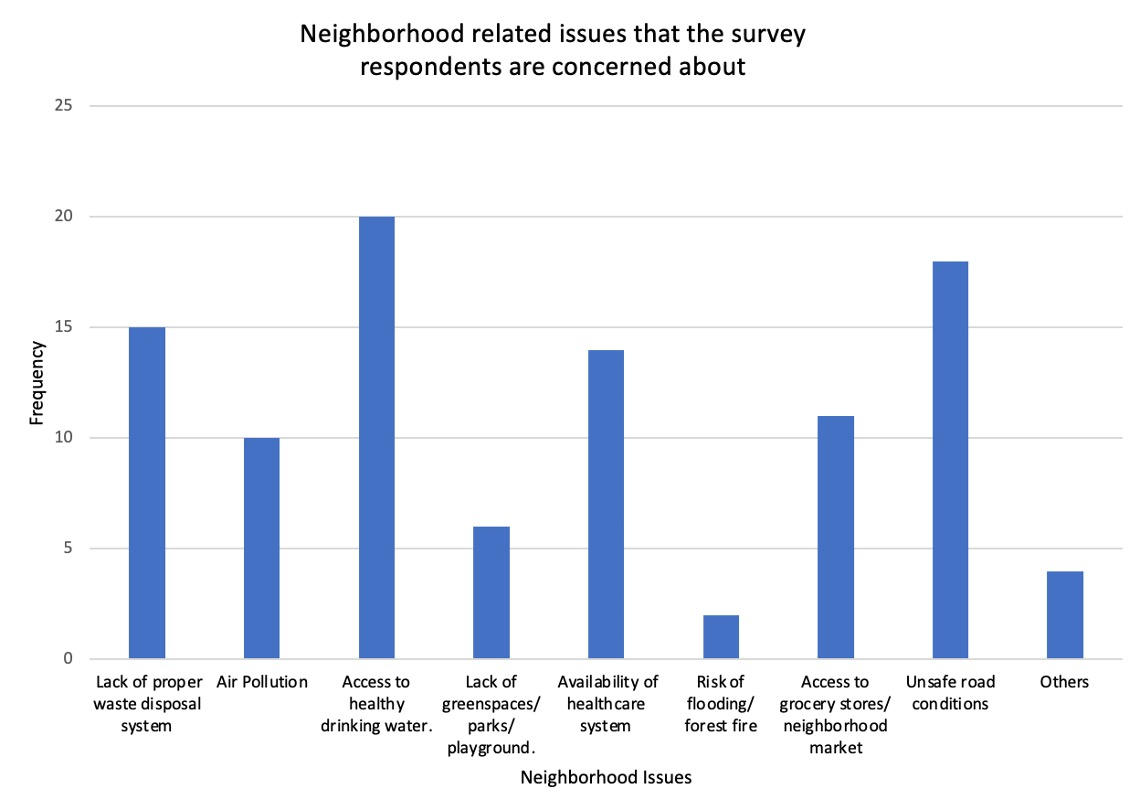
\includegraphics[width=\linewidth]{Bar_new.jpg}
		\caption{Bar graph representing the different neighborhood related issues that the survey respondents are concerned about} 
		\label{fig:Bar}
	\end{figure}
	\paragraph{How to create a bar graph?}
   A bar graph is usually drawn to graph categorical data. To create a bar graph,
    \begin{enumerate}[label=(\alph*), noitemsep]
			\item
	First, create a frequency distribution table, where you will note how many times a particular category has been repeated or the given values corresponding to different categories. For example, question 2 of the "Neighborhood welfare survey" asked the respondents to indicate all the neighbourhood-related issues they were concerned about. The question provided the respondents with nine options. Each option would form one category. The survey response suggests that 20 respondents expressed their concern about access to healthy drinking water. Hence the frequency corresponding to "access to healthy drinking water" is 20. 
	\begin{figure}[h!]
		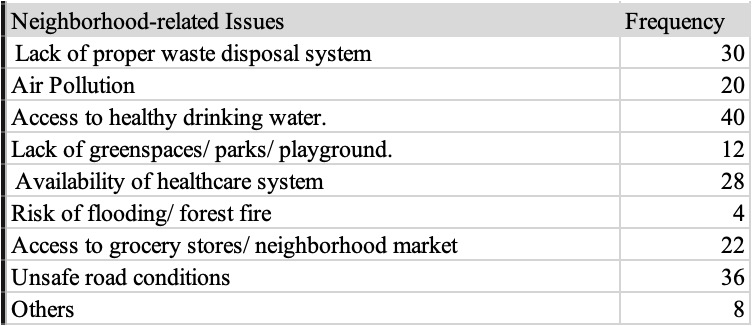
\includegraphics[width=\linewidth]{Freq_dist.jpg}
		\caption{Frequency distribution table of neighborhood-related issues} 
	\end{figure}
	\item
	Next, draw the two axes. Along the horizontal axis, plot all the categories, and along the vertical axis mark the frequencies. 
	\item
	Draw the bars for each category. Note that the height of a bar corresponding to a category is same as its frequency.
			\end{enumerate}
%
	\paragraph{Histogram:} Histogram is a visual tool used to explore the frequency distribution of quantitative data (both Interval and Ratio). The shape of a histogram decides if the data distribution is symmetric or skewed (right skewed and left skewed).\\[1ex]
	The histogram given in Figure~\ref{fig:Hist}, represents the frequency distribution of the “annual household income”. In this histogram, the data has been used to create five bins of size \$5,000 along the $x$-axis, and the frequency of responses has been recorded along the $y$-axis. The important thing to know about a histogram is that the taller the bars are, the greater the frequency they represent. That means, in the given histogram, since the height of the first bin is the highest, 20 to be exact, you can conclude that 20 respondents said that their annual household income is between \$30,000 and \$35,000. 
	\begin{figure}[h!]
		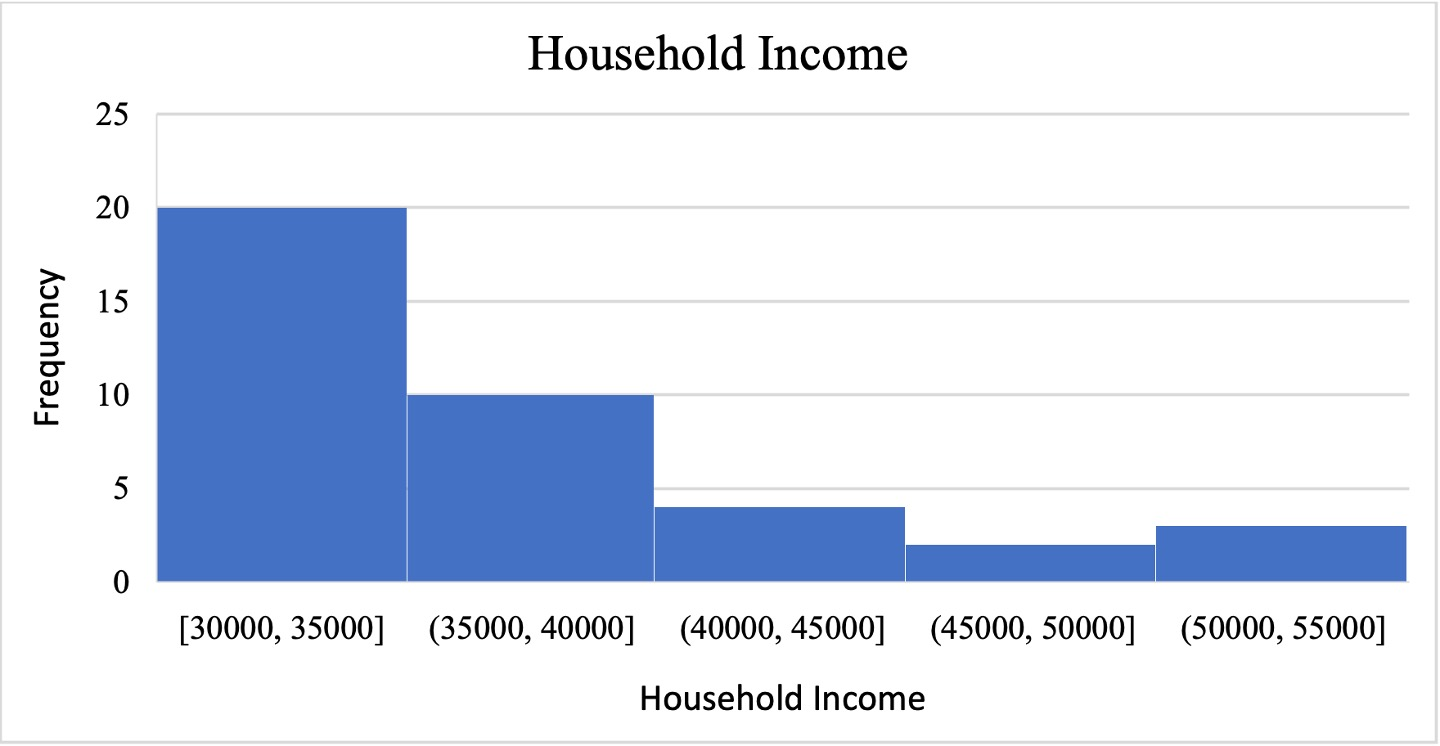
\includegraphics[width=\linewidth]{Hist_new.jpg}
		\caption{Histogram representing the frequency distribution of annual household income of the survey respondents}
		\label{fig:Hist}
	\end{figure}
			\paragraph{How to create a Histogram?}
			To explore the distribution of a quantitative data through a histogram, divide the quantitative data into ordered groups, otherwise known as bins, and count the number of data points that fall in each bin. For example, question 8 of the "Neighborhood welfare survey" asked the respondents about their annual household income. Thirty nine respondents responded to the question. The minimum recorded data is \$30,000, and the maximum recorded data is \$55,000. To create the histogram, 
			\begin{enumerate}[label=(\alph*), noitemsep]
			\item
			First, divide the range of data (\$55,000-\$30,000) into different bins of a fixed size (say \$5,000). So, the bins would be, [30,000-35,000], (35,000-40,000],(40,000-45,000],(45,000-50,000],(50,000-55,000].
			\item
			Next, create a frequency distribution table to count the number of responses that fall under each bin.
			\item
			After the frequency distribution table is prepared, draw two axes. Along the horizontal axis, draw the bins and mark frequencies along the vertical axis. 
			\item
			Finally, draw bars from the lower value of one interval to the lower value of the next interval. The height of each bar should be equal to the frequency of its corresponding interval. That is, in the "Neighborhood welfare survey", if twenty respondents said that their annual household income is between \$30,000 and \$35,000, then the height of the bar corresponding to the bin [30,000-35,000] would be 20.
			\end{enumerate}
	\textbf{\underline{Histogram vs Bar graph:}} Although a histogram looks like a bar graph, there exists a fundamental difference between the two. 
	\begin{enumerate}[label=(\alph*), noitemsep]
		\item 
				A bar graph visually represents categorical data (nominal and ordinal), whereas a histogram represents quantitative data. 
		\item 
				In a bar graph, different categories are represented along the horizontal axis (if the bar graph is oriented vertically), and the associated values are represented along the vertical axis. On the contrary, in a histogram, the horizontal axis represents the different bins of equal length, and the vertical axis represents the frequency of data. 
		\item 
				Since each bar in a bar graph represents different categories, the orders of the bars are not important, and there exist spaces between the consecutive bars. However, in a histogram, the bins are created to organize the quantitative data, so the bins are organized in ascending order, and no gaps exist between any two bins.
	\end{enumerate}
%	
	\paragraph{Box plot:} A box plot, otherwise known as a box and whisker plot, is a visual tool that uses the five-number summary of a data set to look at the spread and distribution of data. The five-number summary of a data set includes its minimum value, lower quartile $ (Q_1)$, median $(Q_2)$, upper quartile $(Q_3)$, and maximum value.\\[1ex]
	\begin{figure}[h!]
		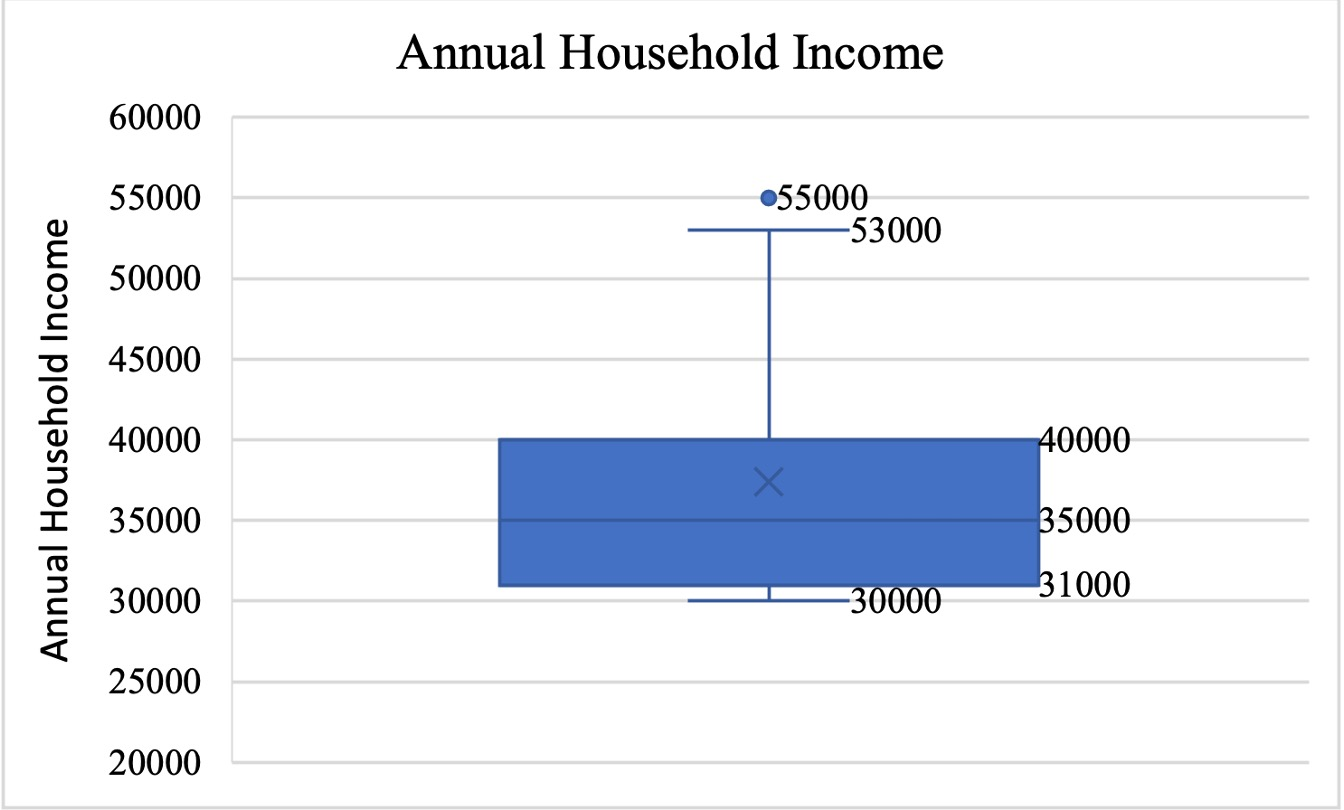
\includegraphics[width=\linewidth]{Boxplot_new.jpg}
		\caption{Box plot representing the annual household income the survey respondents} 
		\label{fig:boxplot}
	\end{figure}
	The box and whisker plot given in Figure~\ref{fig:boxplot} represents the annual household income of the survey respondents.\\[1ex]
	The box in the middle shows the inter-quartile range $(Q_3 – Q_1)$, which contains the middle 50\% of the data. It means, 50\% of the respondents said that their annual household income is between \$31,000 and \$40,000.\\[1ex]	
	The lower and upper whiskers represent the bottom and top 25\% of the responses, respectively. That means 25\% of the respondents said that their annual household income is lower than \$31,000 (lower whisker), and 25\% of the respondents said that their annual household income is more than \$40,000 (Upper whisker).\\[1ex]
	The line in the middle of the box represents the median. It passes through point \$35,000 which indicates that 50\% of the respondents said that their annual household income is more than \$35,000, and 50\% of the respondents said that their annual household income is less than \$35,000.\\[1ex]
	There exists an outlier in the data set. One respondent said that their annual household income is \$55,000, significantly higher than the rest of the responses.
	\paragraph{How to create a Boxplot?}
			To draw a boxplot follow the following steps: 
			\begin{enumerate}[label=(\alph*), noitemsep]
			\item
			First, organize the data in an ascending order. For example, to draw the boxplot of annual household income, first organize the incomes in an ascending order, with the lowest annual household income on the left and the highest annual household income on the right.
			\item
			Next, calculate the median annual household income.\\[1ex]
			\{\textbf{Median}: Median is the middle number in a sorted data set. It divides a data set into exactly two halves, such that 50\% of the data points are lesser than the median, and 50\% of the data points are larger than the median. If the median annual household income is \$35,000, that means 50\% respondents' annual household income is more than \$35,000, and 50\% respondents' annual household income is less than \$35,000\}
			\item
			Next, calculate the first and third quartile.\\[1ex]
			\{\textbf{Quartiles:} Values that divide a data set into four equal parts (quarters) are called quartiles.\\[1ex]
			\textbf{First quartile/ lower quartile:} The first quartile or the lower quartile (Q1) is the data point below which 25\% of the data points, and above which 75\% of the data points are located. If the first quartile of the annual household income data is \$31,000, then 25\% of the respondents' annual household income is less than and 75\% of the respondents' annual household income is more than\$31,000. \\[1ex]
			\textbf{Third quartile/ upper quartile:} The third quartile or the upper quartile (Q3) is the data point below which 75\% of the data points, and above which 25\% of the data points are located. If the third quartile of the annual household income data is \$40,000, then 75\% of the respondents' annual household income is less than and 25\% of the respondents' annual household income is more than\$40,000.\\[1ex]
				\begin{figure}[h!]
		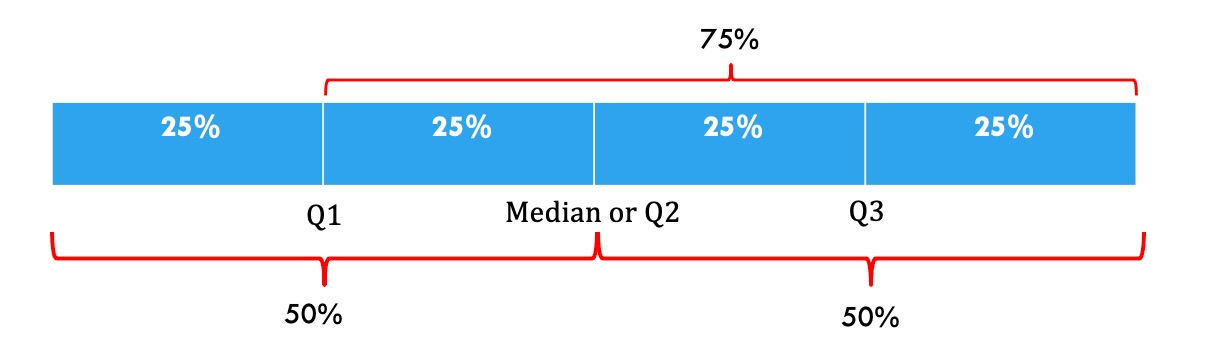
\includegraphics[width=\linewidth]{Quartile.jpg}
		\caption{Figure showing how Quartiles split a data set into four equal parts.} 
	\end{figure}
			\textbf{Interquartile range:} The difference between the third and first quartile is known as interquartile range ($(Q_3 – Q_1)$).\\[1ex]
			\textbf{Outliers:} An outlier is an observation (data point), which is either too high or too low compared to the rest of the data points in a data set. For example, in the annual household income data set, the annual household income of \$55,000 is an outlier. That means, the respondent having an annual household income of \$55,000 is earning considerably high compared to the rest of the respondents who filled the survey.\\[1ex]
			\textbf{Finding an outlier:} The rule that is followed to identify an outlier in a given data set is called 1.5 x IQR. When a data set is given, 
			\begin{enumerate}[label=(\alph*), noitemsep]
			\item
			First find its median, upper quartile, and the lower quartile. 
			\item
			Next, calculate the value of interquartile range $(Q_3-Q_1)$
			\item
			Calculate 1.5 x IQR = 1.5 x $(Q_3-Q_1)$
			\item
		    Find the fences:\\[1ex]
		    Upper fence: $Q_3$ + 1.5 x $(Q_3-Q_1)$
		    Lower fence: $Q_1$ - 1.5 x $(Q_3-Q_1)$
		    \item
		    Any data point beyond the fences, that is either lower than the lower fence or higher than the upper fence is an outlier\}
				\end{enumerate}
			\item
			Finally, draw a number line (horizontal or vertical) and use the five number summaries, minimum value, lower quartile $ (Q_1)$, median $(Q_2)$, upper quartile $(Q_3)$, and maximum value, to draw the box and whisker plot.
			\begin{figure}[h!]
		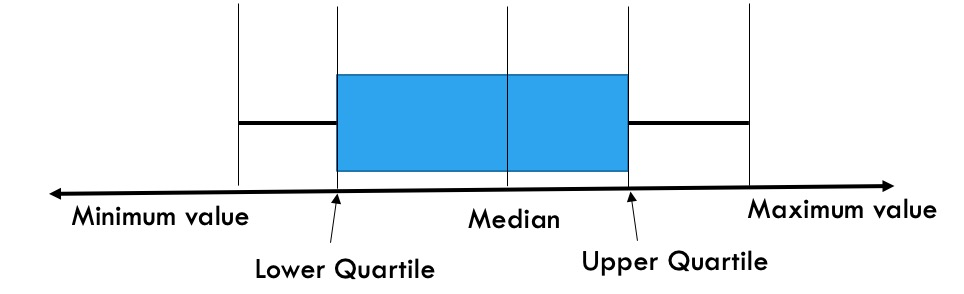
\includegraphics[width=\linewidth]{draw_box.jpg}
		\caption{Figure showing how to draw a box plot when there is no outlier} 
	\end{figure}
			If there exists one or more outlier in a data set, then the rule will be slightly different. If there is an outlier on the lower side, then to draw the lower whisker join the lower quartile and the lowest non-outlier data point. If there is an outlier on the upper side, then to draw the upper whisker join the upper quartile and the highest non-outlier value. 
			\end{enumerate}
%
	\paragraph{Scatter plot:} A scatter plot is a visual tool that is used to visualize the relationship between two numeric variables. In a scatter plot, the independent variable is usually plotted along the horizontal or $x$-axis, and the dependent variable is usually plotted along the vertical or $y$-axis.\\[1ex]
	\begin{figure}[h!]
		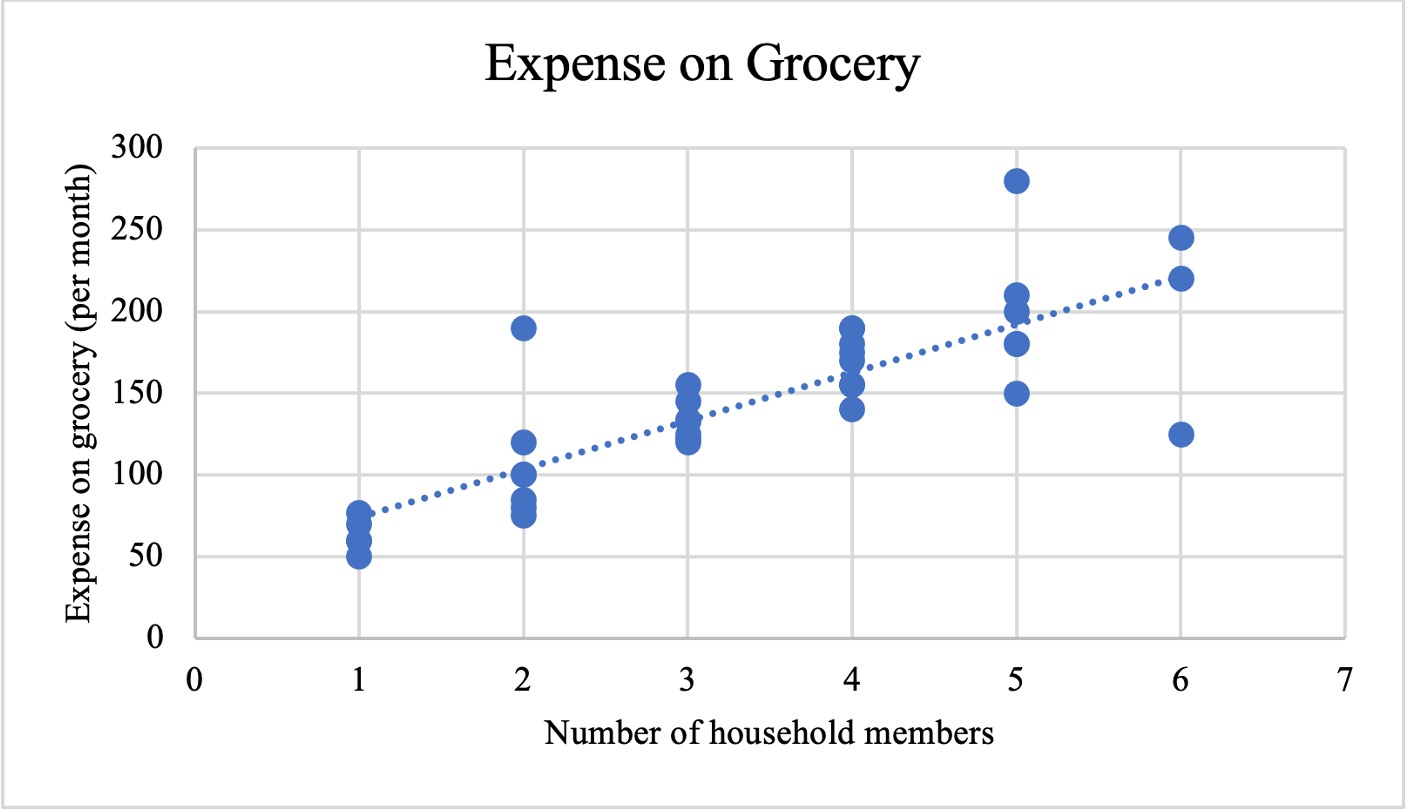
\includegraphics[width=\linewidth]{scatter_new.jpg}
		\caption{Scatter plot representing the relationship between the number of household members of the survey respondents and their monthly grocery expenses} 
		\label{fig:scatter}
	\end{figure}
%	
	The scatter plot given in Figure ~\ref{fig:scatter} represents the relationship between the  \emph{number of household members of the survey respondents} and their  \emph{monthly grocery expenses}. As the figure suggests, the variable  \emph{number of household members} is an independent variable (plotted along the $x$-axis), and the variable  \emph{monthly grocery expense} is a dependent variable (plotted along the $y$-axis). The scatter plot shows if there exists a relationship between the two variables, that is if the number of household members impacts the respondents’ monthly grocery expenses.
	\paragraph{How to create a scatter plot?}
			Scatter plots are drawn to explore the correlation between two variables. One variable (independent variable) is considered an explanatory variable, and the other is considered a dependent variable. For example, in the "Neighborhood welfare survey", respondents were asked about their number of household members and their monthly grocery expenses. If someone explores the possible impact of the number of household members on monthly grocery expenses, then the number of household members would be considered an independent variable, and monthly grocery expenses would be a dependent variable (depends on the number of family members). To draw a scatter plot,
			\begin{enumerate}[label=(\alph*), noitemsep]
			\item
			Identify the independent and dependent variables.
			\item
			Plot independent variable along the horizontal axis or x-axis, and plot the dependent variable along the vertical axis or y-axis. Label the axes.
			\item
			Plot the ordered pairs (idependent variable, dependent variable)
			\end{enumerate}
			Three types of linear correlation can be identified through the patterns displayed by a scatterplot.
			\begin{enumerate}[label=(\alph*), noitemsep]
			\item
			Positive correlation: If the increase/ decrease in one variable indicates an increase/ decrease in the other variable, then there exists a positive correlation between the two variables. 
			\begin{figure}[h!]
			\centering
		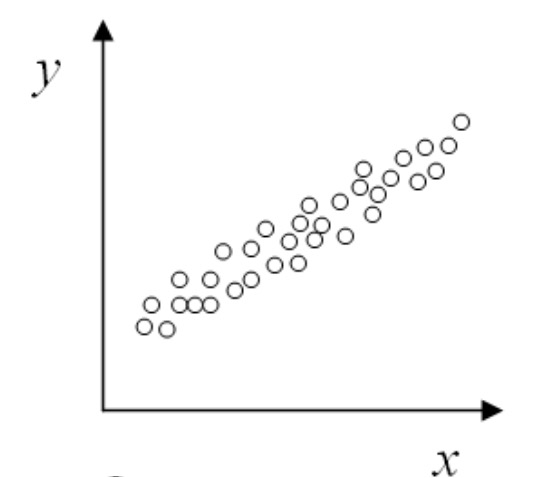
\includegraphics[width=9 cm, height=9cm]{Positive cor.jpg}
		\caption{Scatter plot indicating a positive correlation between two variables.Source: \href{https://en.wikipedia.org/wiki/File:Strong--weak--no-correlation.png}{Wikipedia} is licensed with \href{https://creativecommons.org/licenses/by-sa/3.0/deed.en}\href{https://creativecommons.org/licenses/by-sa/2.5/deed.en}} 
	\end{figure}
			\item
			Negative correlation: If the increase/ decrease in one variable indicates an decrease/ increase in the other variable, then there exists a negative correlation between the two variables. 
			\begin{figure}[h!]
			\centering
		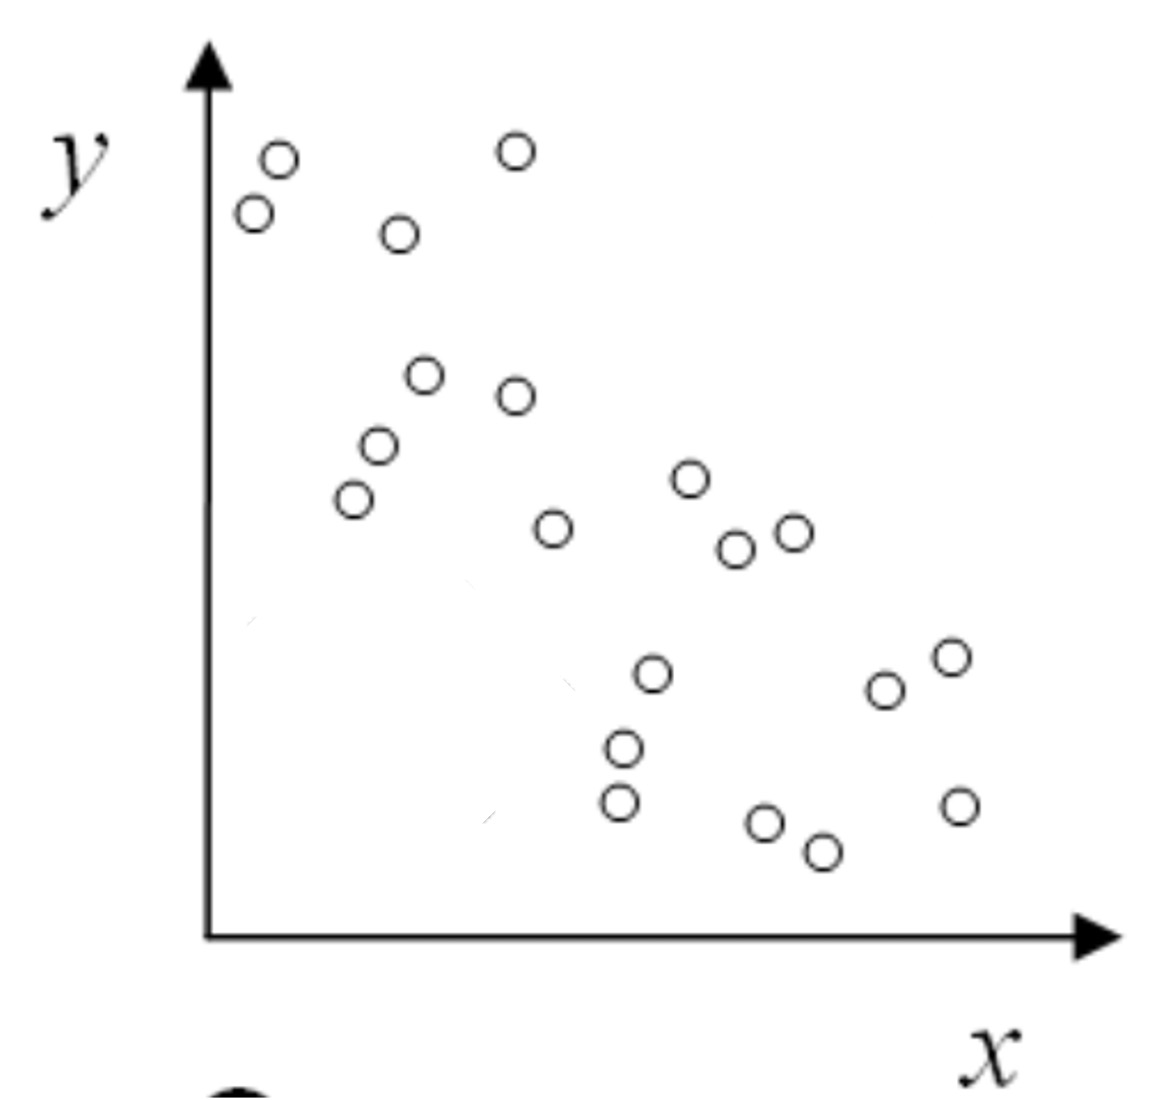
\includegraphics[width=9cm, height=9cm]{neg_cor.jpg}
		\caption{Scatter plot indicating a negative correlation between two variables.Source: \href{https://en.wikipedia.org/wiki/File:Strong--weak--no-correlation.png}{Wikipedia} is licensed with \href{https://creativecommons.org/licenses/by-sa/3.0/deed.en}\href{https://creativecommons.org/licenses/by-sa/2.5/deed.en}} 
	\end{figure}
			\item
			No correlation: 
			\begin{figure}[h!]
			\centering
		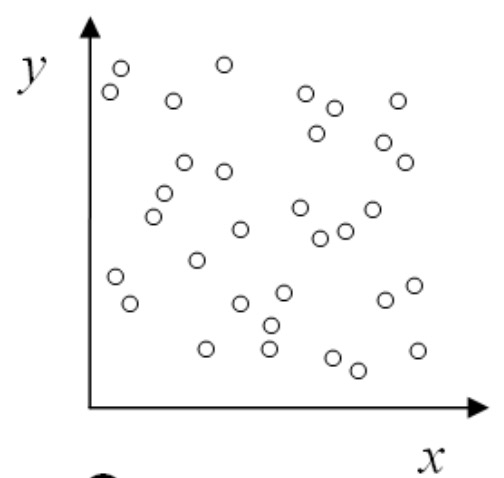
\includegraphics[width=9cm, height=9cm] {no_Corr.jpg}
		\caption{Scatter plot indicating no correlation correlation between two variables.Source: \href{https://en.wikipedia.org/wiki/File:Strong--weak--no-correlation.png}{Wikipedia} is licensed with \href{https://creativecommons.org/licenses/by-sa/3.0/deed.en}\href{https://creativecommons.org/licenses/by-sa/2.5/deed.en}} 
	\end{figure}
			\end{enumerate}
%
%
%Section 4: Solving for Change
%
%
\section{Solving for change}
%
%
%
Now that we have discussed data types and data visualization, we can begin to explore how the unfavorable living conditions in the Cancer Alley have made its residents, particularly impoverished people of color, more vulnerable to medical conditions with disproportionate health facilities. Watch the video: \href{https://www.youtube.com/watch?v=MGNtMkFJkKg}{Cancer risk in Louisiana town nearly 50 times higher than national average} and share your thoughts on the following questions:
	\begin{enumerate}[label=\alph*), itemsep=0.5ex]
		\item 
		Were you familiar with the Cancer Alley?
		\item 
        		How did you feel as you watched the conditions of the people living on the Cancer Alley?
        		\item 
        		Who do you think is most affected by the chemical factories located in the region? Why?
        \end{enumerate}
         Next, form groups of two and explore the data given in Worksheet 3: Racial distribution of the cities and parishes on the Cancer Alley. The data set contains information about the different parishes along the Cancer Alley, their racial compositions, median household incomes, and access to hospitals and medical facilities.\\[1ex]
         As you explore the data, answer the following questions:
         \begin{enumerate}[label=\alph*), itemsep=0.5ex]
		\item 
      		Which of the given variables in the data set collected categorical data?
         	\item 
         	Which of the given variables in the data set collected quantitative data?
         	\item 
		What visualization would you choose to compare the percentage of African American population and the White population in the different parishes along the Cancer Alley? Justify your answer.
		\item 
		Go to Excel and draw a visualization to compare the percentage of African American population and the White population in the different parishes along the Cancer Alley. Interpret your findings.
		\item 
		Draw an appropriate visualization to explore the distribution of median household income (2016-2020) in the different parishes along the Cancer Alley? What is the nature of the distribution? Explain. 
		\item 
		What visualization would help you investigate the possible impact of median household income on the number of hospitals in the different parishes along the Cancer Alley? Draw the visualization and interpret your findings. 
	\end{enumerate}
%
%
%Subsection 4.1: In-depth Exploration
%
\subsection{In-depth Exploration}
%
	Construct one research question that you intend to answer using the given data. You must choose at least one form of data visualization to answer your research question and justify your choice of data visualization (I decided to construct a scatter plot because I want to explore the correlation between two quantitative data).\\[1ex]
	After you complete working on the problem, create a short presentation (PowerPoint or poster) and present their findings to the whole class. The presentation should contain the following points:
	\begin{enumerate}[label=\alph*), itemsep=0.5ex]
		\item 
		Brief introduction to the problem (problem statement/ significance of your topic)
	\item 
		Research Question
\item 
		Data Visualization
\item 
		Results/ Data Interpretations
\item 
		Conclusion
	\end{enumerate}
%
%
%Section 5: Summary
%
\section{Summary or Reading Questions}
%
%
	In this last section of the chapter, engage in a whole-class discussion and reflect on the long-lasting environmental justice issue in the Cancer Alley. Consider the following questions to engage in the discussion:
	\begin{enumerate}[label=\alph*), itemsep=0.5ex]
		\item Did any of the findings surprise you?
		\item How does this lesson impact your understanding of systemic environmental discrimination?
		\item Ask the students to explore the location of chemical factories, hazardous waste facilities, and oil refineries in their local regions (neighborhood, towns, cities, state). Calculate the distance of those facilities from the nearest schools and residential areas (Google map or field trip), and investigate if those facilities have had any health impact on local residents.
	\end{enumerate}
%
%
%Section 6: Exercise
%
%
\section{Exercise}
%
	\begin{enumerate}[font=\bfseries]
		\item 
				Interpret the histogram given in \vref{Hist_Cancer} on distribution of number of days from +ve COVID confirmation to clinical recovery.
				\begin{figure}
					\begin{minipage}{\linewidth}
						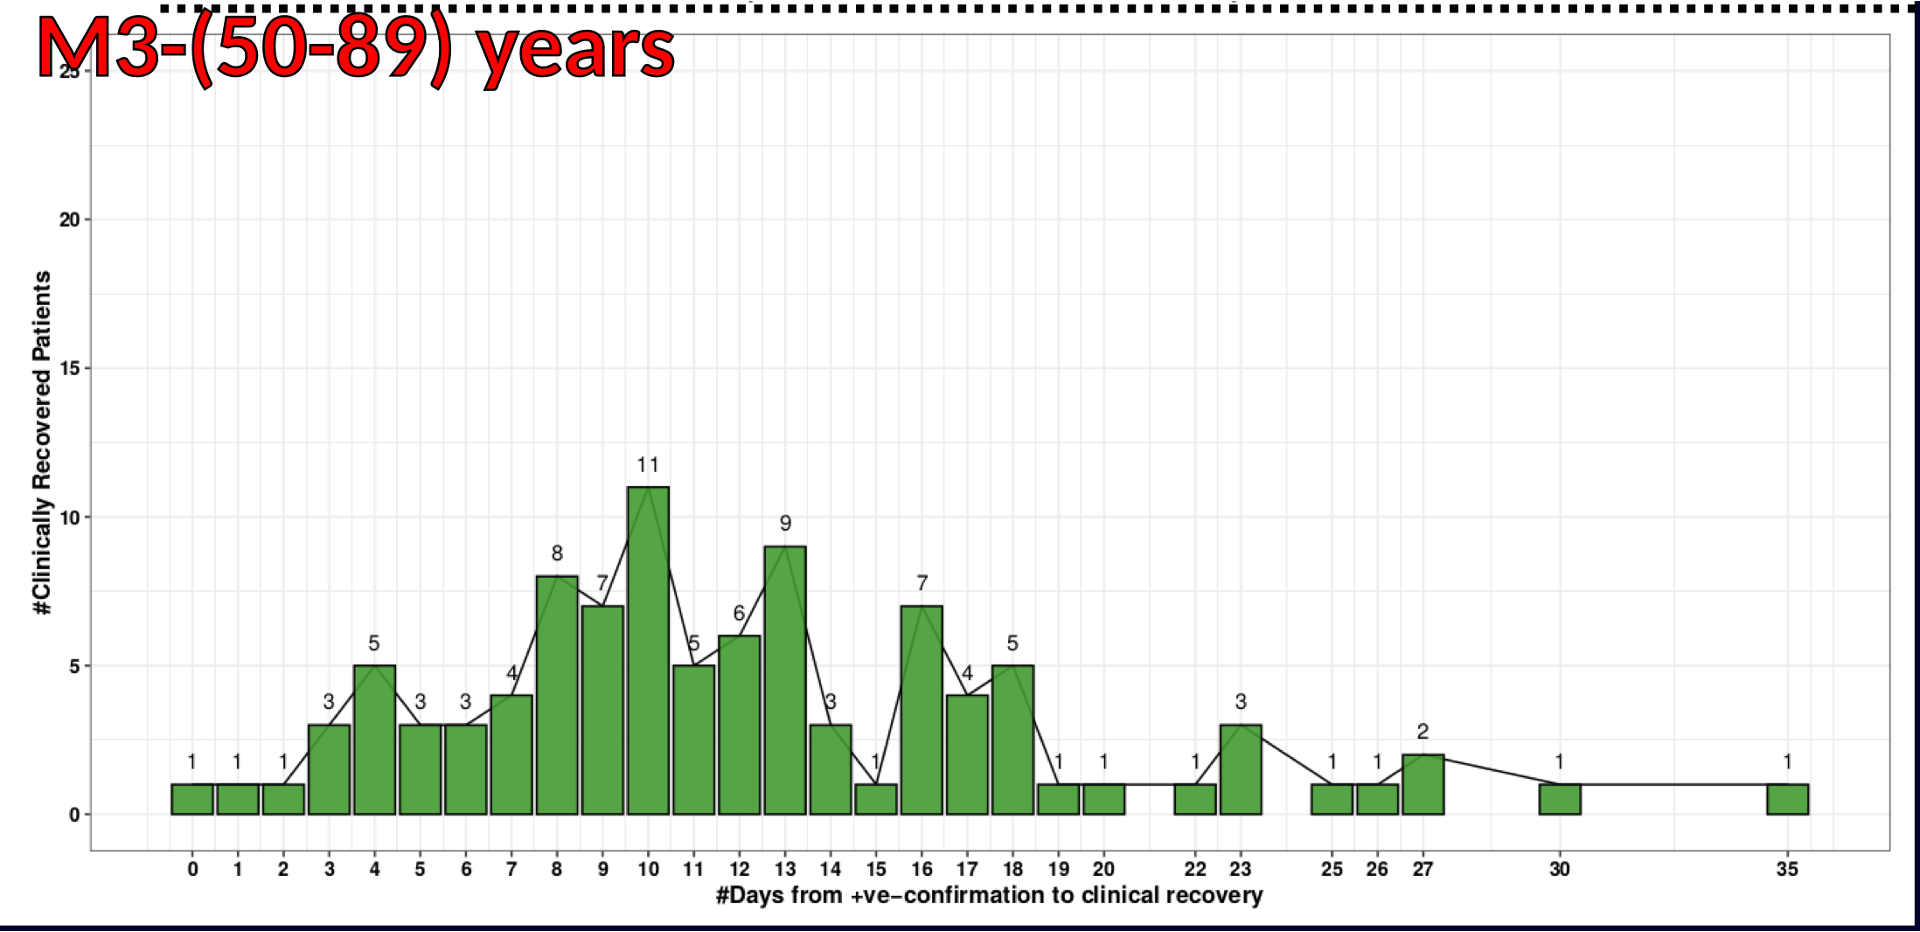
\includegraphics[width=\linewidth]{Hist_Cancer.png}
						\caption{Histogram showing patient-count distribution of number of days from +ve COVID confirmation to clinical recovery in Singapore during January 23-April 01.\protect\footnote{Source: Sreevalsan-Nair, J., Vangimalla, R. R., \& Ghogale, P. R. (2020). Analysis of clinical recovery-period and recovery rate estimation of the first 1000 COVID-19 patients in Singapore. medRxiv}}
						\label{Hist_Cancer}\vspace{5ex}
						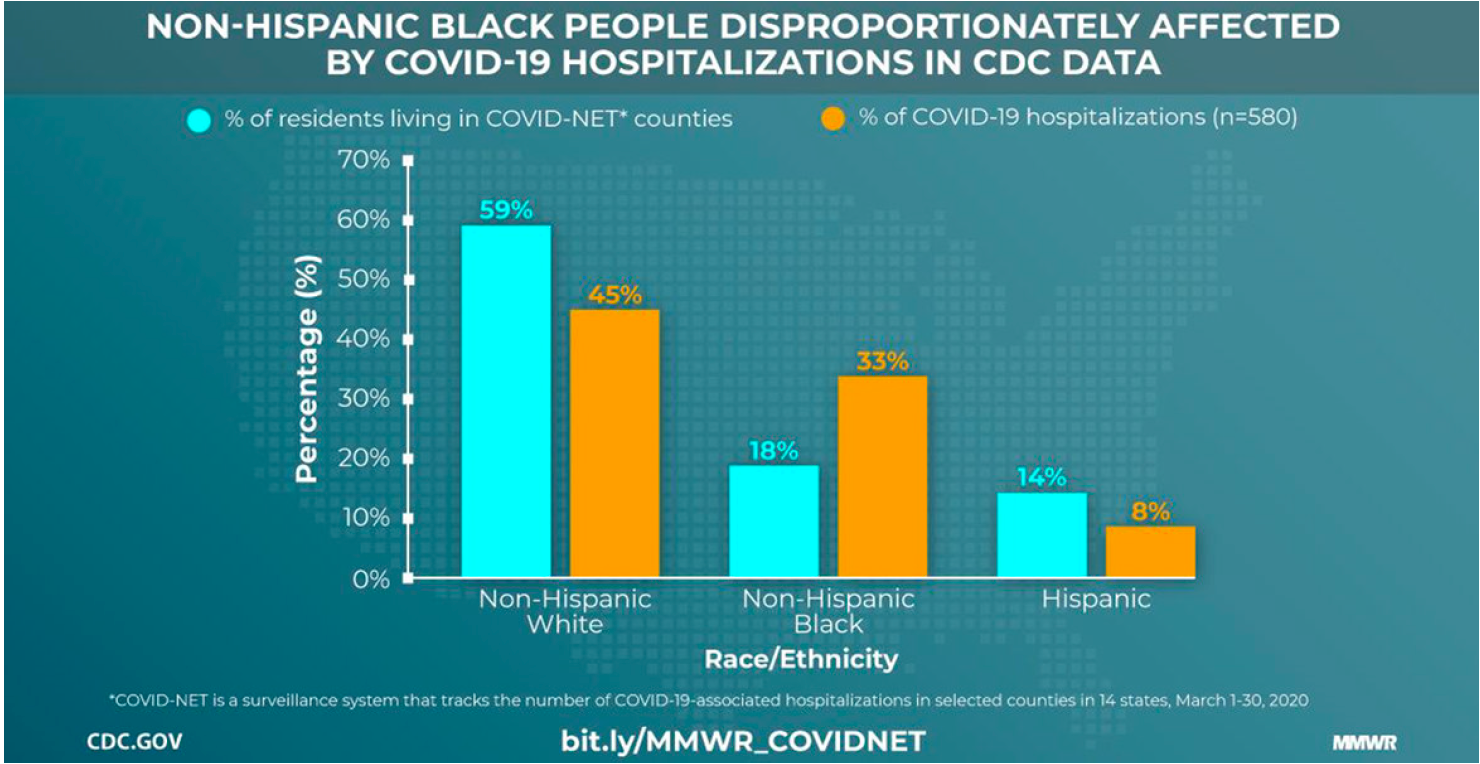
\includegraphics[width=\linewidth]{Bar_Cancer.png}
						\caption{Bar graph showing CDC’s (2020b) data visualization of COVID-19 hospitalizations, broken down by race/ethnicity\protect\footnote{Source: Centers for Disease Control and Prevention. (2020b). Data visualization. Centers for disease control and prevention. Retrieved May 11, 2020, from \url{https://www.cdc.gov/coronavirus/2019-ncov/covid-data/data-visualization.htm}}}
						\label{Bar_Cancer}
					\end{minipage}
				\end{figure}
				\begin{enumerate}[label=\alph*), itemsep=0.5ex]
					\item How many people recovered in four days?
					\item How many people took twenty-three days to recover?
					\item How many people took eight to thirteen days to recover?
					\item Is there any potential outlier?
				\end{enumerate}
				\begin{figure}[b!]
					\begin{minipage}{\linewidth}
						\includegraphics[width=\linewidth]{Vaccine_Cancer.png}
						\caption{Bar Graph representing the number of COVID-19 vaccine doses as claimed by different countries\protect\footnote{Data as of Nov. 30. Potential dose purchases include deals that are under negotiation and options for additional doses as part of existing confirmed deals. Source: \href{https://launchandscalefaster.org/COVID-19}{Launch and Scale Speedometer, Duke Global Health Innovation Center} \emph{Credit: Connie Hanzhang Jin/NPR}}}
						\label{Vaccine_cancer}
					\end{minipage}
				\end{figure}
		\item 
				Go to the data set \emph{Households by total money income}. The data set has been taken from \href{https://www.census.gov/data/tables/2021/demo/income-poverty/p60-273.html}{U.S. Census Bureau} and simplified for the lesson.
				\begin{enumerate}[label=\alph*), itemsep=0.5ex]
					\item How has the estimated median income (dollar) of white people changed from 2002 to 2020?
					\item How has the estimated median income (dollar) of black people changed from 2002 to 2020?
					\item What visualization would be most appropriate to explore the change of the estimated median income over the years?
					\item Make at least two interpretations from the visualizations about the change of the white and black people's estimated median income.
				\end{enumerate}
		\item 
				Go to the data set \emph{Households by total money income}. The data set has been taken from \href{https://www.census.gov/data/tables/2021/demo/income-poverty/p60-273.html}{U.S. Census Bureau} and simplified for the lesson.
				\begin{enumerate}[label=\alph*), itemsep=0.5ex]
					\item Compare the estimated median income (dollar) of the White, Black, Asian, and Hispanic people from 2002 to 2020. 
					\item What visualization would be most appropriate to compare the estimated median income of the four racial groups?
					\item Make at least two interpretations from the visualization(s) and report how the estimated median income of one racial group is different from others.
				\end{enumerate}
		\item 
				Interpret the bar graph given in \vref{Bar_Cancer} on COVID-19 hospitalizations, broken down by race/ethnicity.
		\item 
				Interpret the bar graph in \vref{Vaccine_cancer} on COVID-19 vaccine doses as claimed by different countries and answer the following questions:
				\begin{enumerate}[label=\alph*), itemsep=0.5ex]
					\item Which country has definitively purchased the maximum number of COVID vaccine doses? 
					\item Which country is speculated to have contained the maximum number of CODID vaccine doses?
					\item The total population of the USA is approximately 328 million. If the USA contains 2.6 billion vaccine doses, how many times can it vaccinate its population, if most COVID vaccines require individuals to take two doses to protect themselves from the virus?
					\item The total population of Canada is approximately 38 million. If Canada contains 414 million vaccine doses, how many times can it vaccinate its population, if most COVID vaccines require individuals to take two doses to protect themselves from the virus?
				\end{enumerate}
	\end{enumerate}
%
%
%
%
%
%	
%
%
%
%
%
%
%
\begin{thebibliography}{}
	\bibitem{BRD18}Bullard, R. D. (2018). \emph{Dumping in Dixie: Race, class, and environmental quality}. Routledge.
	\bibitem{BRD19}Bullard, R. D. (2019). Environmental blackmail in minority communities. \emph{In Race and the incidence of environmental hazards} (pp. 82-95). Routledge.
	\bibitem{CIG21}Castellón, I. G. (2021). Cancer Alley and the Fight Against Environmental Racism. \emph{Vill. Envtl. LJ}, 32, 15.
	\bibitem{SM11}Singer, M. (2011). Down cancer alley: The lived experience of health and environmental suffering in Louisiana's chemical corridor. \emph{Medical Anthropology Quarterly}, 25(2), 141-163.
\end{thebibliography}
%
%
%
%

%
%
\newpage
\subsection*{Worksheet 3}
%
\newcolumntype{M}[1]{>{\small\centering\arraybackslash}m{#1\textwidth}}
	\begin{table}[h!]
		\centering
		\setlength\tabcolsep{0pt}
		\def\arraystretch{1}
		\begin{tabular}{|*{11}{M{0.1}|}}
			\hline\hline
			Place/ Parish\tablefootnote{Table provides statistics for all states and counties, and for cities and towns with a \emph{population of 5,000 or more}} 
%			
			& Population Estimates\tablefootnote{Sources: U.S. Census Bureau, Population Estimates Program (PEP), updated annually. \href{https://www.census.gov/programs-surveys/popest.html}{Population and Housing Unit Estimates}} 
%			
			& White alone, percent\tablefootnote{\label{f7}Includes persons reporting only one race}
%			
			& Black or African American alone, percent\footref{f7}
%			
			& Hispanic or Latino, percent\tablefootnote{Hispanics may be of any race, so also are included in applicable race categories}
%			
			& Asian alone, percent\footref{f7}
%			
			& Native Hawaiian or Pacific Highlander alone, percent\footref{f7}
%			
			& American Indian, or Alaska Native alone, percent\footref{f7}
%			
			& Median Household Income (in 2020 dollar) 2016-2020\footref{f7}
%			
			& Number of Hospitals\footref{f7}
%			
			& Number of Hospitals (per capita)\footref{f7}\\
			\hline\hline
			Batton Rouge	&	2,20,236	&	38.7	&	54.7	&	3.7	&	3.5	&	0.1	&	0.3	&   \$44,177	&	28	&	38\\
			\hline
			St. Gabriel (Iberville Parish)	&	7,460	&	31	&	67.5	&	1.9	&	0.1	&	0	&	0.4 &	\$52,103	&	2	&	40\\
			\hline
			Plaquemine city (Iberville)	&	6,539	&	43	&	54.9	&	6.4	&	0	&	0	&	0	&	\$51,750	&	2	&	40	\\
			\hline
			Reserve (St. John the Baptist)	&	9,280	&	35	&	60.6	&	7.4	&	0.2	&	0	&	0	&	\$42,120	&	2	&	47	\\
			\hline
			Laplace (St. John the Baptist Parish)	&	29,147	&	41.4	&	52.1	&	6.8	&	1.6	&	0	&	0	&	\$55,429	&	2	&	47	\\
			\hline
			St. James Parish, LA	&	21,096	&	49.7	&	48.8	&	1.8	&	0.4	&	0	&	0.3 &	\$53,209	&	2	&	24	\\
			\hline
			Gonzales (Ascension Parish)	&	10,957	&	36.9	&	51.5	&	10	&	2.1	&	0	&	0	&	\$82,594	&	4	&	58	\\
			\hline
			St. Charles Parish, LA	&	53,100	&	70.2	&	26.5	&	6.4	&	1.1	&	0.1	&	0.4 &	\$68,113	&	2	&	56	\\
			\hline\hline
		\end{tabular}
		\caption{Racial distribution of the cities and parishes on the cancer alley\tablefootnote{Source: QuickFacts data are derived from: Population Estimates, American Community Survey, Census of Population and Housing, Current Population Survey, Small Area Health Insurance Estimates, Small Area Income and Poverty Estimates, State and County Housing Unit Estimates, County Business Patterns, Non-employer Statistics, Economic Census, Survey of Business Owners, Building Permits.\url{https://www.census.gov/quickfacts/fact/table/batonrougecitylouisiana/PST045219}}}
		\label{W3}
	\end{table}
%
%
%
%
%
%
%
\end{document}